\documentclass[12pt]{article}
\usepackage[utf8]{inputenc}
\usepackage[french]{babel}
\usepackage[T1]{fontenc}
\usepackage{graphicx}
\usepackage[export]{adjustbox} 
\usepackage{geometry}
\usepackage{tabularx}
\usepackage[most]{tcolorbox}
\usepackage{enumitem}
\usepackage{listings}
\usepackage[table]{xcolor}
\usepackage{amssymb} 
\usepackage[hidelinks]{hyperref}
\usepackage{fancyhdr} 
\usepackage{float} 
\usepackage{caption} 
\captionsetup[figure]{font=it}
% Configuration pour le bloc JSON
\lstset{
    basicstyle=\ttfamily\small,
    breaklines=true,
    frame=single,
    backgroundcolor=\color{gray!5},
    literate={é}{{\'e}}1 {è}{{\`e}}1 {à}{{\`a}}1 
}
\graphicspath{{images/}}
\geometry{a4paper, margin=2cm, top=1.5cm, bottom=3cm}
% --- CONFIGURATION DU PIED DE PAGE ---
\pagestyle{fancy}
\fancyhf{} 
\renewcommand{\headrulewidth}{0pt} 
\renewcommand{\footrulewidth}{0.5pt} 
\fancyfoot[L]{\small \textbf{Tp services web}}
\fancyfoot[R]{\small \textbf{Page \thepage}}

\begin{document}

% --- PAGE DE GARDE ---
\thispagestyle{empty} 
\noindent
\begin{tabularx}{\textwidth}{@{} c >{\centering\arraybackslash}X c @{}}

\includegraphics[width=3.5cm, valign=t]{logoujkz.jpeg} & 
\begin{minipage}[t]{\linewidth}
    \centering
    \small \textbf{UNIVERSITÉ JOSEPH KI-ZERBO} \\
    \small *********** \\
    \small UNITÉ DE FORMATION ET DE RECHERCHE \\
    \small EN SCIENCES EXACTES ET APPLIQUÉES \\
    \small ********** \\
    \small \textbf{DÉPARTEMENT INFORMATIQUE (Master 1)} \\
    \small Année académique 2025-2026
\end{minipage} & 

\includegraphics[width=4.5cm, valign=t]{ufr.png} 
\end{tabularx}
\vspace{0.5cm}
\hrule height 1pt
\vspace{1.5cm}
\begin{center}
    \begin{tcolorbox}[
        enhanced,
        width=0.85\textwidth,
        colback=orange!5!white, 
        colframe=brown!80!black,
        arc=0pt,
        boxrule=1.2pt,
        underlay={
            \path[draw=brown!80!black, line width=1.2pt, 
                  left color=brown!50!orange!30, right color=orange!5!white, middle color=white] 
                ([xshift=-15pt, yshift=5pt]frame.north west) 
                arc[start angle=180, end angle=540, x radius=10pt, y radius=5pt] 
                -- ([xshift=5pt, yshift=-5pt]frame.south west)
                arc[start angle=360, end angle=0, x radius=10pt, y radius=5pt] 
                -- cycle;
            \path[draw=brown!80!black, line width=1.2pt, 
                  right color=brown!50!orange!30, left color=orange!5!white, middle color=white] 
                ([xshift=15pt, yshift=5pt]frame.north east) 
                arc[start angle=0, end angle=-360, x radius=10pt, y radius=5pt] 
                -- ([xshift=-5pt, yshift=-5pt]frame.south east)
                arc[start angle=-180, end angle=180, x radius=10pt, y radius=5pt] 
                -- cycle;
        },
        shadow={1.5mm}{-1.5mm}{0mm}{black!30!white},
        halign=center,
        top=0.8cm,
        bottom=0.8cm,
        left=0.8cm,
        right=0.8cm
    ]
        \vspace{0.2cm}
        {\Huge \textbf{\textsc{Rapport : Services Web}}} \\
        \vspace{0.5cm}
        {\large \textit{TP -- Conception et utilisation d'un service REST}} \\
        \vspace{0.2cm}
    \end{tcolorbox}
\end{center}
\vfill 
\noindent
\begin{tabularx}{\textwidth}{@{} X >{\raggedleft\arraybackslash}X @{}}
    \textbf{Enseignant :} & \textbf{Membres du groupe :} \\
    Dr. SOMBDA & GNISSIEN Migouel \\
               & TAPSOBA Sandrine Pelagie\\
\end{tabularx}

\newpage 

% --- TABLE DES MATIÈRES ---
\renewcommand{\contentsname}{Table des matières}
\tableofcontents 
\newpage 

% --- LISTE DES FIGURES ---
\listoffigures 
\addcontentsline{toc}{section}{Liste des figures}
\newpage 

% --- INTRODUCTION ---
\section*{Introduction}
\addcontentsline{toc}{section}{Introduction}
Le développement moderne des applications distribuées repose en grande partie sur l'échange de données entre systèmes hétérogènes. Dans ce contexte, les services web et l'architecture REST se sont imposés comme des standards incontournables grâce à leur simplicité et leur scalabilité. Ce rapport présente les travaux réalisés dans le cadre du cours de Master 1. L'étude se concentre sur la mise en place d'une architecture conforme aux bonnes pratiques, notamment par l'utilisation d'URI sémantiques et la manipulation rigoureuse des verbes HTTP fondamentaux. Nous abordons ainsi les opérations de création, de lecture et de suppression, tout en approfondissant la gestion des modifications via les méthodes PUT et PATCH, ainsi que des fonctionnalités avancées de validation et de pagination.
\newpage 

\section{Partie 1 --- Modélisation REST}
\subsection{Identification des ressources}
L'architecture du système repose sur une modélisation orientée ressources, où le \textbf{Cours} constitue l'entité pivot autour de laquelle gravitent les interactions des autres composants du domaine. Les ressources identifiées pour ce système sont les suivantes :
\begin{itemize}
    \item \textbf{Cours}
    \item \textbf{Étudiant}
    \item \textbf{Enseignant}
    \item \textbf{Inscription}
\end{itemize}

\subsection{Définition des URI et Verbes HTTP}
\begin{center}
\renewcommand{\arraystretch}{1.8}
\begin{tabularx}{\textwidth}{|l|l|X|}
\hline
\rowcolor{orange!5!white} \textbf{Action prévue} & \textbf{Méthode} & \textbf{Point de terminaison (URI)} \\ \hline
\multicolumn{3}{|c|}{\textbf{Cours}} \\ \hline
Lister les cours & GET & /api/cours \\ \hline
Lire un cours & GET & /api/cours/\{id\_cours\} \\ \hline
Créer un cours & POST & /api/cours \\ \hline
Modifier un cours & PUT & /api/cours/\{id\_cours\} \\ \hline
Modifier partiellement & PATCH & /api/cours/\{id\_cours\} \\ \hline
Supprimer un cours & DELETE & /api/cours/\{id\_cours\} \\ \hline
\multicolumn{3}{|c|}{\textbf{Étudiants}} \\ \hline
Lister les étudiants & GET & /api/etudiants \\ \hline
Lire un étudiant & GET & /api/etudiants/\{id\_etudiant\} \\ \hline
Créer un étudiant & POST & /api/etudiants \\ \hline
Modifier un étudiant & PUT & /api/etudiants/\{id\_etudiant\} \\ \hline
Supprimer un étudiant & DELETE & /api/etudiants/\{id\_etudiant\} \\ \hline
\multicolumn{3}{|c|}{\textbf{Enseignants}} \\ \hline
Lister les enseignants & GET & /api/enseignants \\ \hline
Lire un enseignant & GET & /api/enseignants/\{id\_enseignant\} \\ \hline
Créer un enseignant & POST & /api/enseignants \\ \hline
Modifier un enseignant & PUT & /api/enseignants/\{id\_enseignant\} \\ \hline
Supprimer un enseignant & DELETE & /api/enseignants/\{id\_enseignant\} \\ \hline
\multicolumn{3}{|c|}{\textbf{Inscriptions}} \\ \hline
Lister les inscriptions & GET & /api/inscriptions \\ \hline
Inscrire un étudiant & POST & /api/inscriptions \\ \hline
Supprimer une inscription & DELETE & /api/inscriptions/\{id\_inscription\} \\ \hline
\multicolumn{3}{|c|}{\textbf{Relations}} \\ \hline
Cours d'un étudiant & GET & /api/etudiants/\{id\_etudiant\}/cours \\ \hline
\end{tabularx}
\end{center}
\vspace{0.5cm}
\noindent \textbf{Justification des choix REST}
\begin{itemize}[label=$\checkmark$]
    \item \textbf{Légèreté et Performance :} Contrairement à SOAP qui utilise du XML lourd, REST privilégie le JSON, réduisant la taille des messages et accélérant le traitement, un atout majeur pour les applications mobiles.
    \item \textbf{Interopérabilité :} En se basant sur le protocole HTTP standard, REST permet à des systèmes totalement différents (Web, Mobile, IoT) de communiquer sans protocoles complexes supplémentaires.
    \item \textbf{Scalabilité :} L'architecture est \textit{stateless} (sans état). Le serveur ne stocke pas de session client, ce qui facilite la montée en charge et la gestion de milliers de requêtes simultanées.
    \item \textbf{Simplicité de mise en \oe uvre :} L'utilisation des verbes HTTP (GET, POST, etc.) rend l'interface intuitive pour les développeurs par rapport aux architectures RPC.
\end{itemize}

\newpage
\section{Partie 2 --- Consommation de l'API}
\noindent \textbf{Note sur la sécurité des identifiants :} \\
Pour la suite des requêtes présentées, nous allons utiliser des \textbf{ID complexes} (mélange de caractères et de chiffres). Contrairement aux identifiants auto-incrémentés simples (1, 2, 3), l'utilisation de chaînes alphanumériques complexes permet de sécuriser l'API en évitant les attaques par énumération de ressources.

\subsection{Création d'un cours (POST)}
\begin{center}
\begin{minipage}{0.8\textwidth}
\begin{lstlisting}
POST /api/cours
{
  "titre": "Architecture Logicielle",
  "enseignant": "Dr. Somda",
  "volumeHoraire": 24,
  "actif": true
}
\end{lstlisting}
\end{minipage}
\end{center}
\begin{figure}[H]
    \centering
    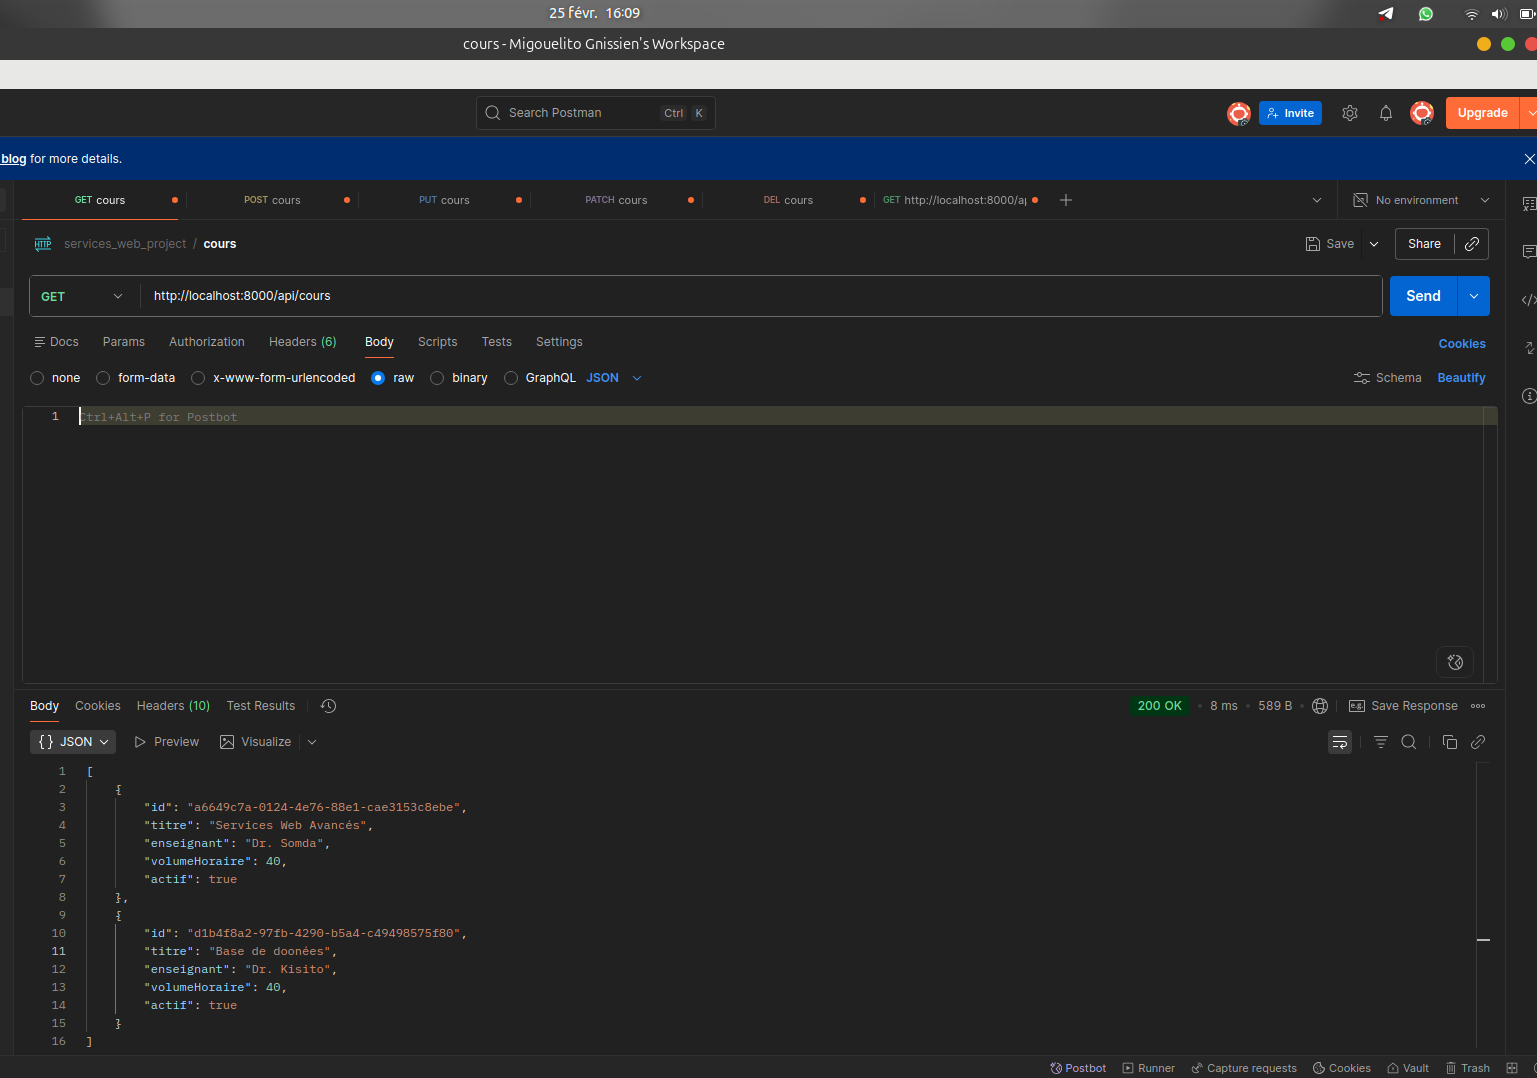
\includegraphics[width=0.95\textwidth]{1.png}
    \caption{Requête POST réussie sous Postman}
\end{figure}

\subsection{Consultation (GET)}
\begin{figure}[H]
    \centering
    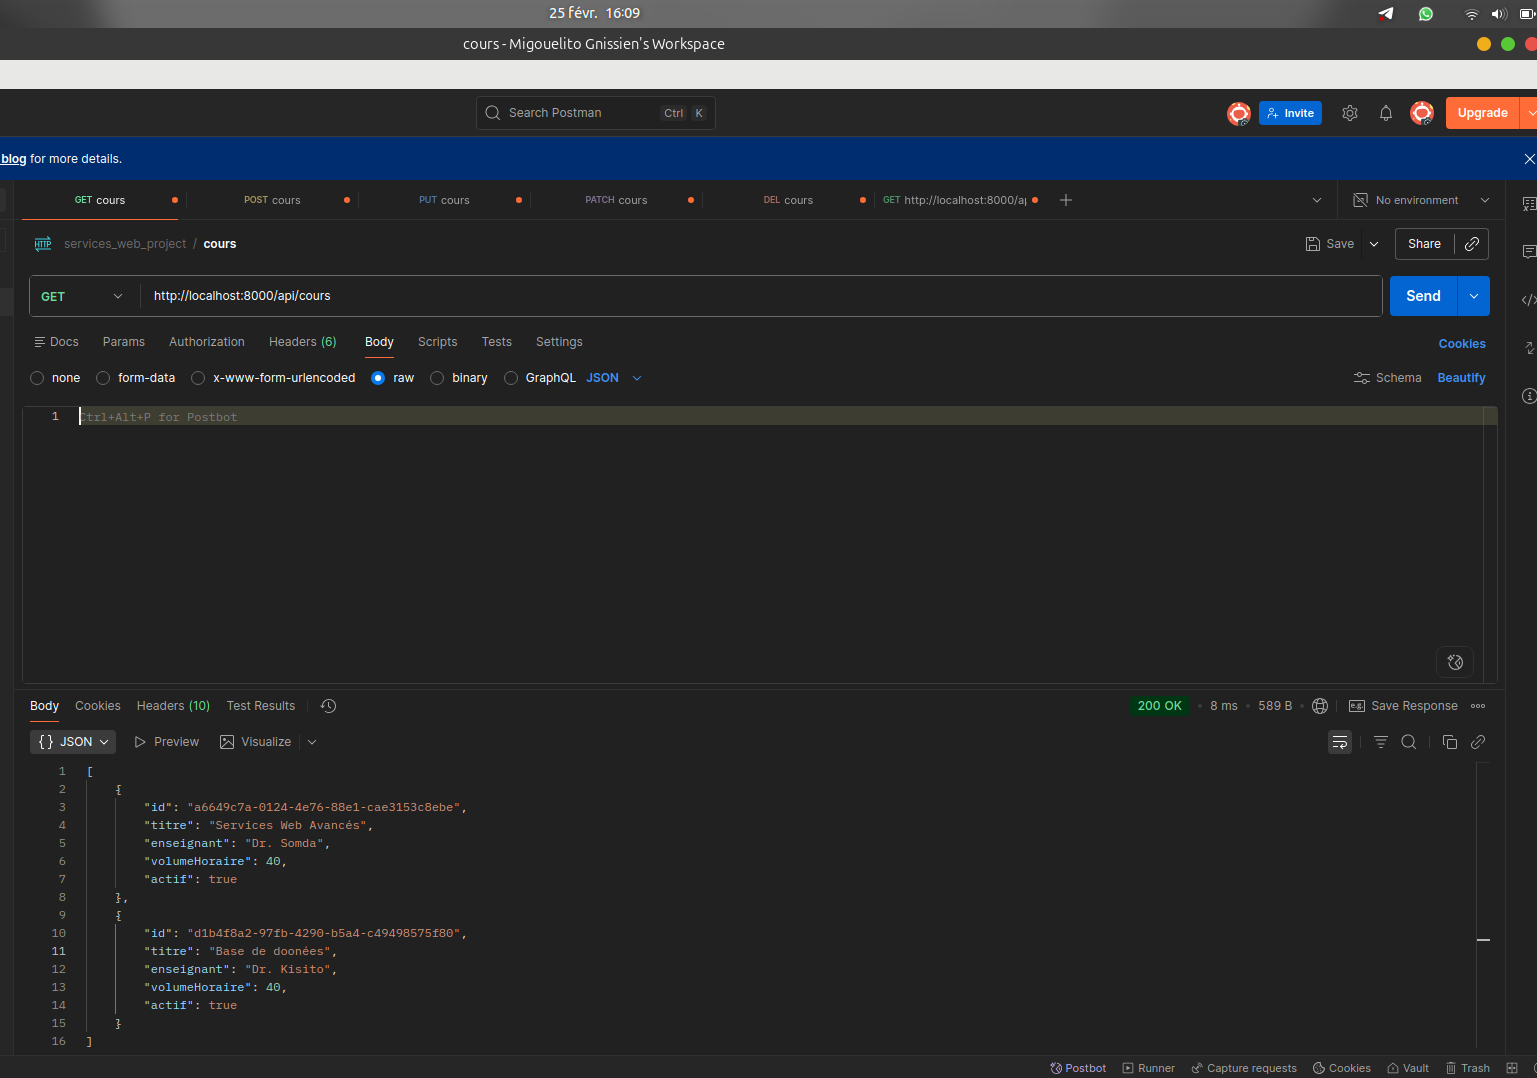
\includegraphics[width=0.95\textwidth]{1.png}
    \caption{Récupération de la collection des cours (GET)}
\end{figure}

\newpage
\section{Partie 3 --- Mise à jour : PUT vs PATCH}
\subsection{PUT (Remplacement complet)}
\begin{center}
\begin{minipage}{0.8\textwidth}
\begin{lstlisting}
PUT /api/cours/1
{
  "id": "7f8b9c2a1-e4d5-4a2b-8c7d-9e0f1a2b3c4d",
  "titre": "Services Web Avancés",
  "enseignant": "Dr. Somda",
  "volumeHoraire": 36,
  "actif": true
}
\end{lstlisting}
\end{minipage}
\end{center}
\begin{figure}[H]
    \centering
    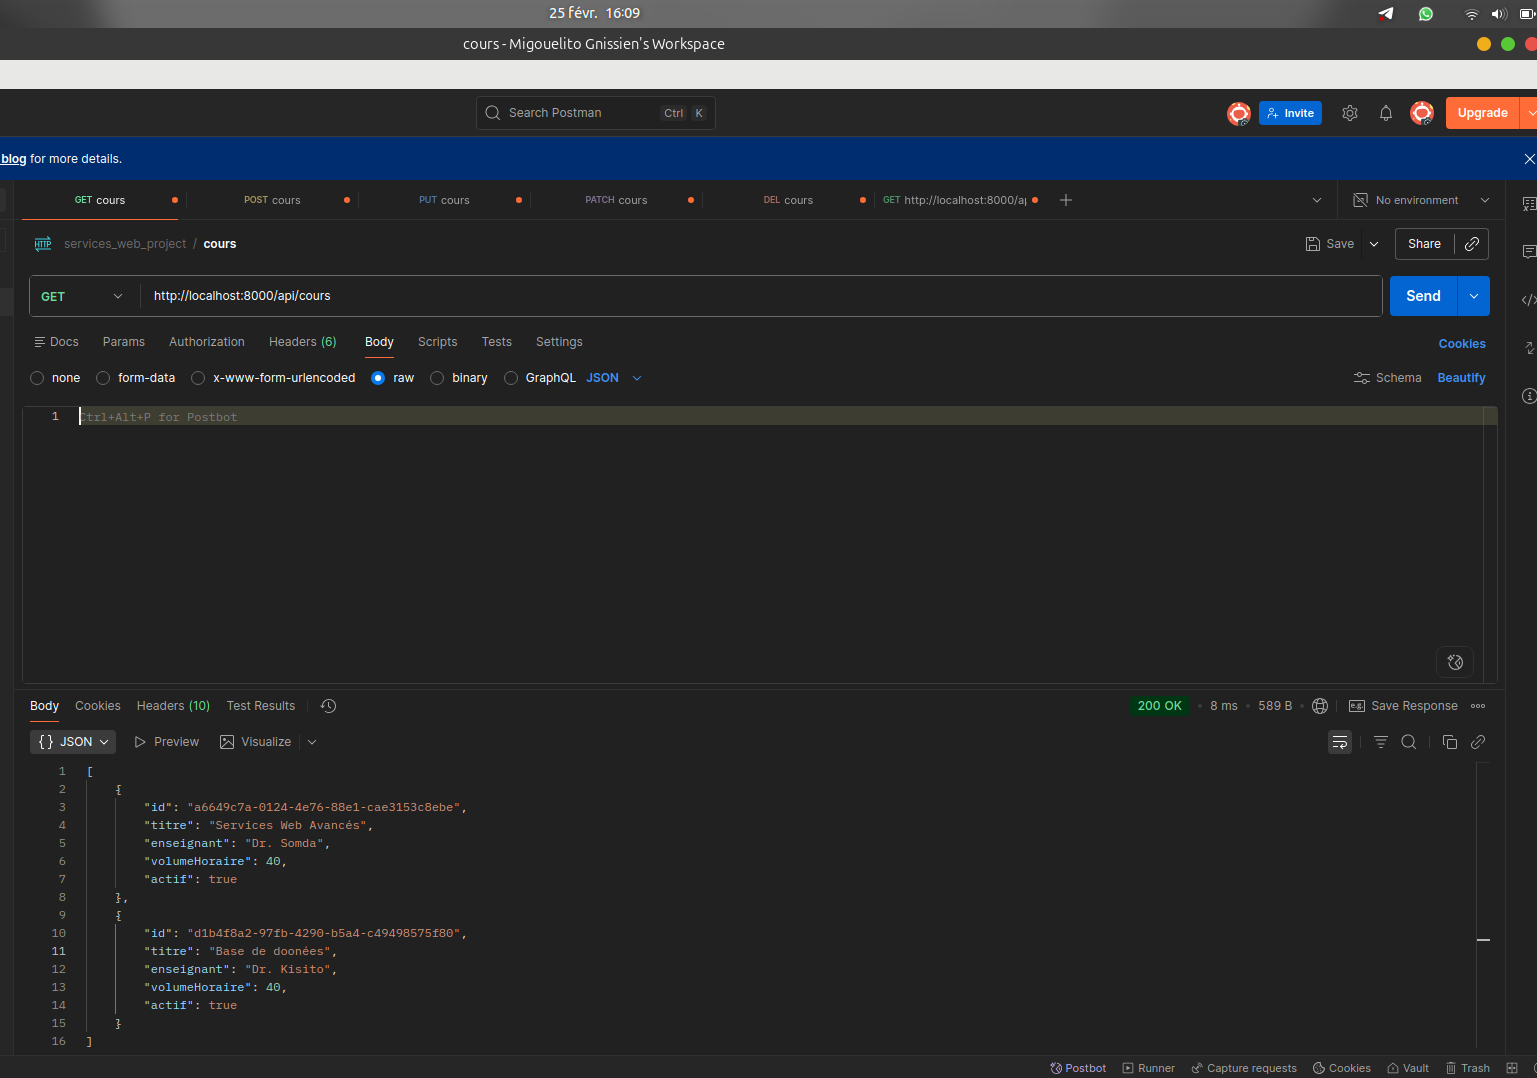
\includegraphics[width=0.95\textwidth]{1.png}
    \caption{Résultat de la mise à jour complète (PUT)}
\end{figure}

\subsection{PATCH (Modification partielle)}
\begin{center}
\begin{minipage}{0.8\textwidth}
\begin{lstlisting}
PATCH /api/cours/1
[
  { "op": "replace", "path": "/volumeHoraire", "value": 40 }
]
\end{lstlisting}
\end{minipage}
\end{center}
\begin{figure}[H]
    \centering
    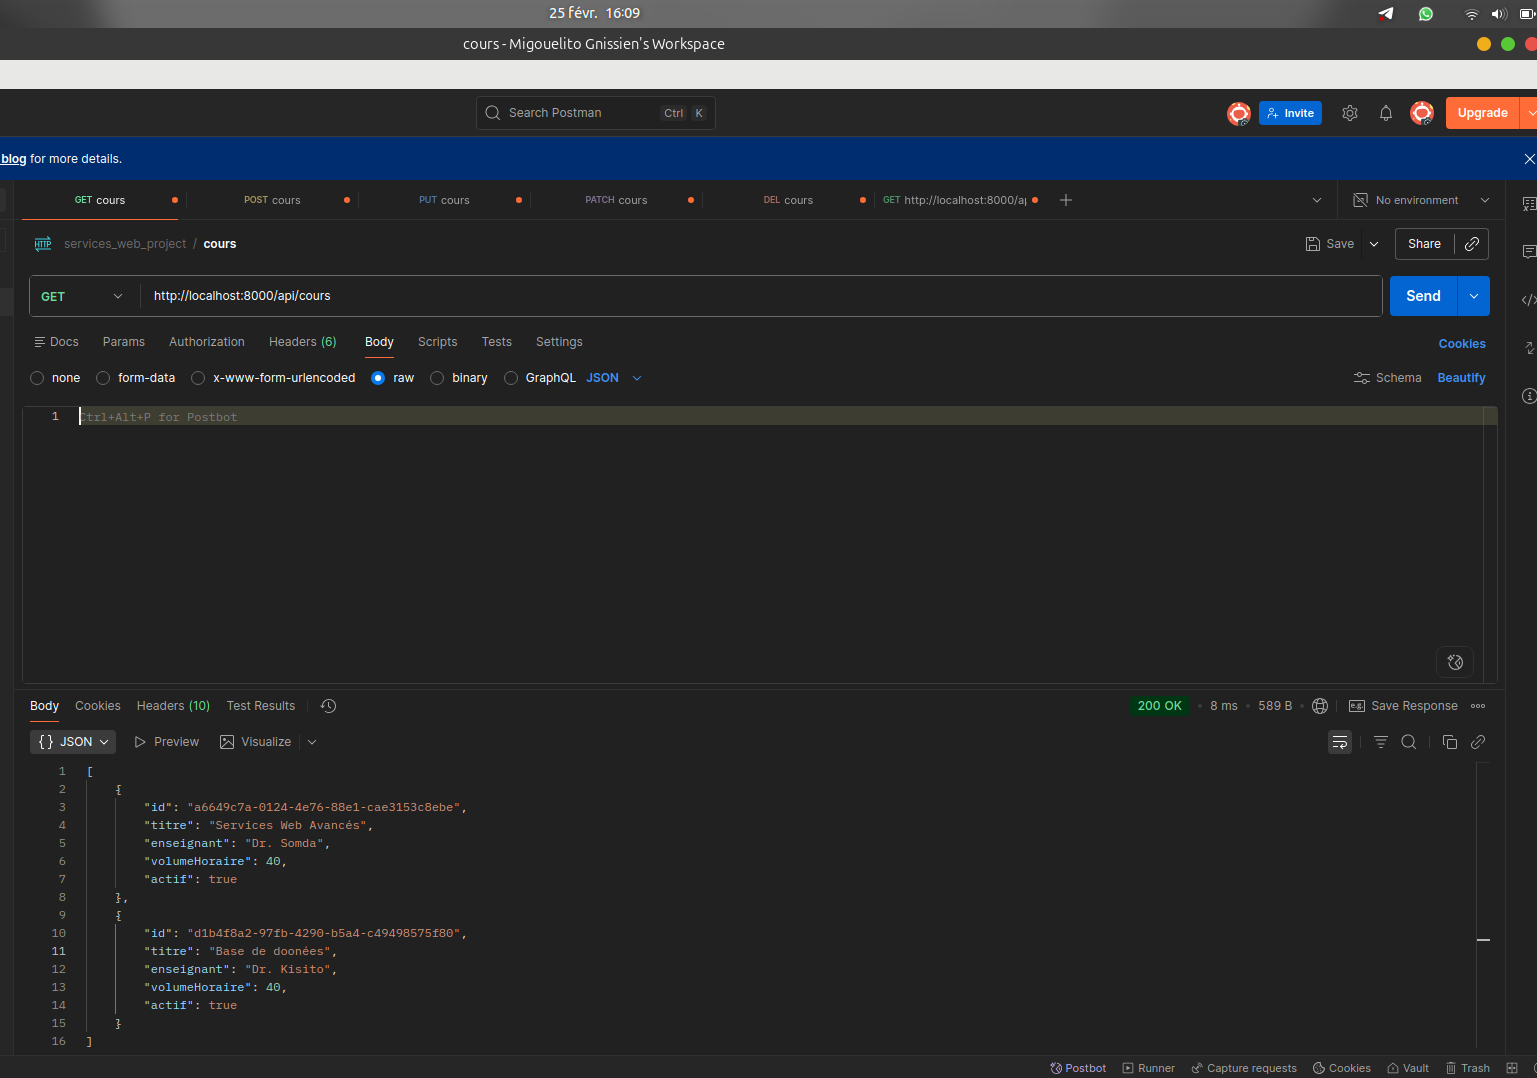
\includegraphics[width=0.95\textwidth]{1.png}
    \caption{Résultat de la modification partielle (PATCH)}
\end{figure}

\newpage
\section{Partie 4 --- Codes HTTP et gestion des erreurs}
\subsection{Exemple d'erreur 404}
\begin{center}
\begin{minipage}{0.8\textwidth}
\begin{lstlisting}
{
  "error": "Cours non trouvé",
  "timestamp": "2026-02-20T10:30:00"
}
\end{lstlisting}
\end{minipage}
\end{center}
\begin{figure}[H]
    \centering
    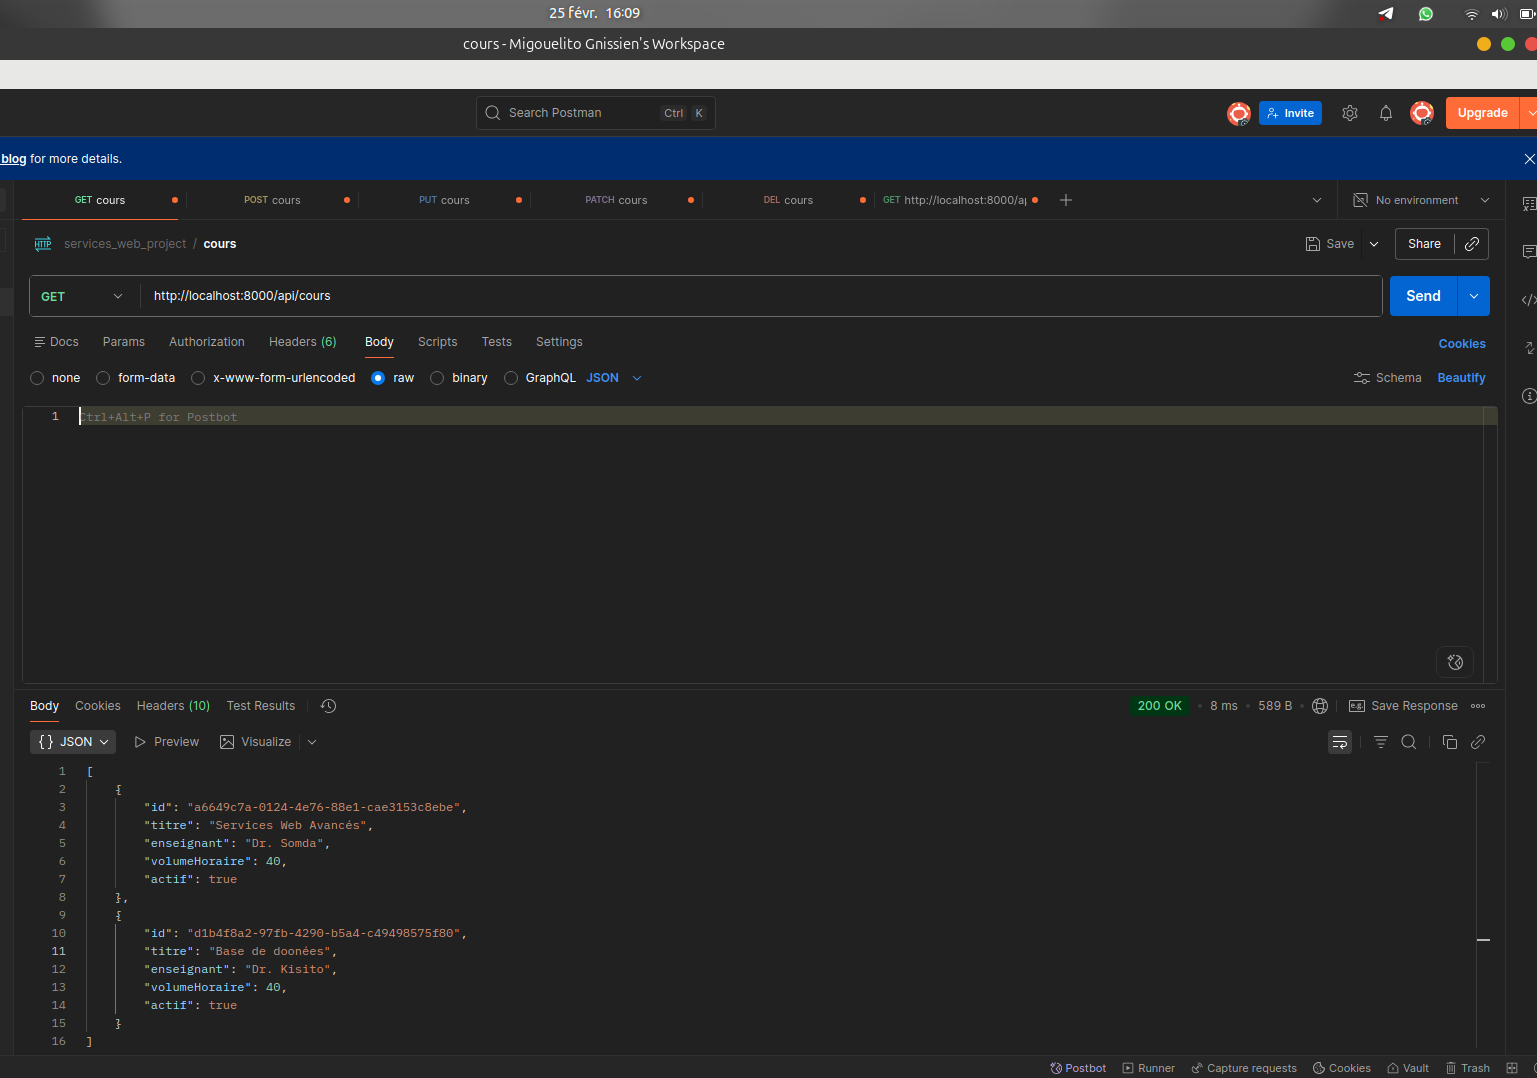
\includegraphics[width=0.95\textwidth]{1.png}
    \caption{Capture d'écran de l'erreur 404 rencontrée}
\end{figure}

\newpage
\section{Partie 5 --- Bonus (Niveau Master)}
\subsection{Validation métier : volumeHoraire > 0}
Une contrainte a été ajoutée pour empêcher l'insertion de volumes horaires incohérents.
\begin{center}
\begin{minipage}{0.8\textwidth}
\begin{lstlisting}
POST /api/cours
{
  "titre": "Test Erreur",
  "volumeHoraire": -10
}
\end{lstlisting}
\end{minipage}
\end{center}
\begin{figure}[H]
    \centering
    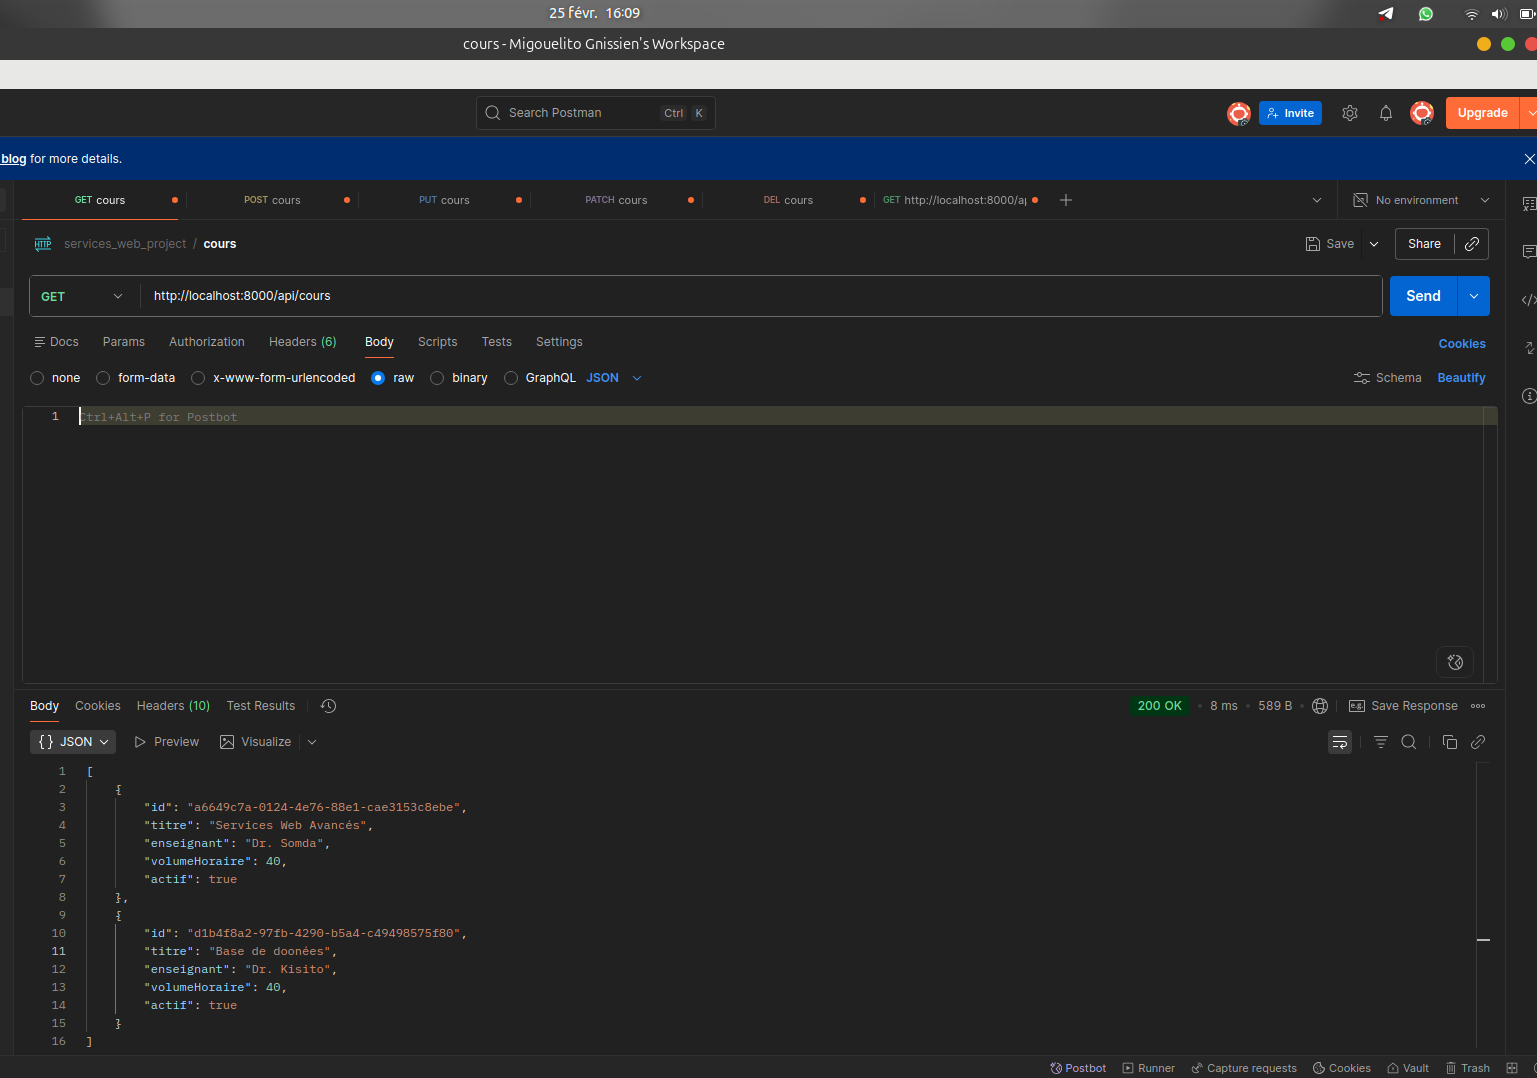
\includegraphics[width=0.95\textwidth]{1.png}
    \caption{Échec de la validation métier}
\end{figure}

\subsection{Pagination des ressources}
Pour optimiser les performances, nous avons implémenté la pagination via les paramètres \texttt{page} et \texttt{size}.
\begin{center}
\begin{minipage}{0.8\textwidth}
\begin{lstlisting}
GET /api/cours?page=0&size=5
\end{lstlisting}
\end{minipage}
\end{center}
\begin{figure}[H]
    \centering
    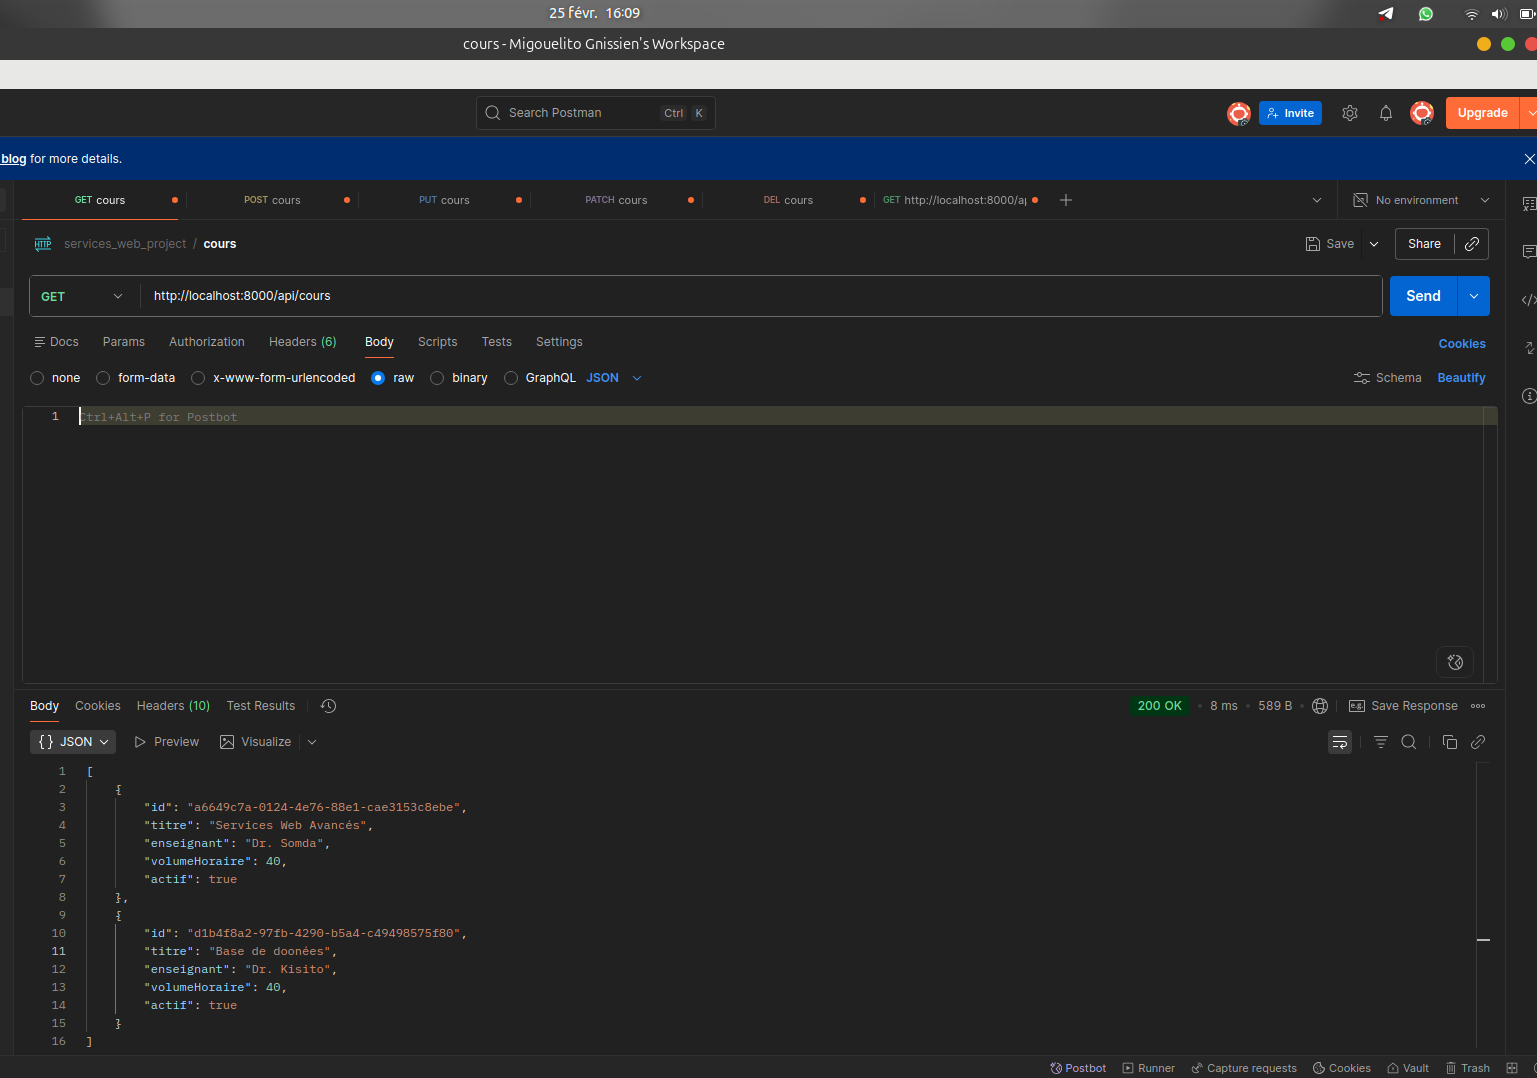
\includegraphics[width=0.95\textwidth]{1.png}
    \caption{Visualisation de la pagination sous Postman}
\end{figure}

\newpage
\section{Technologies Utilisées}
La mise en \oe uvre de ce service web repose sur des outils modernes garantissant rapidité de développement et robustesse des tests.

\vspace{0.8cm}
\noindent \textbf{Langage Python :} Utilisé pour sa syntaxe concise et sa large bibliothèque standard, idéal pour le traitement de données et la logique métier.
\begin{figure}[H]
    \centering
    
\includegraphics[width=0.95\textwidth]{python.png}
    \caption{Logo du langage Python}
\end{figure}

\vspace{0.4cm}
\noindent \textbf{Framework Django :} Nous avons exploité Django REST Framework pour construire l'API. Son architecture robuste permet une séparation claire entre les modèles de données et les contrôleurs.
\begin{figure}[H]
    \centering
    
\includegraphics[width=0.95\textwidth]{django.png}
    \caption{Logo du Framework Django REST}
\end{figure}

\vspace{0.4cm}
\noindent \textbf{Base de données PostgreSQL :} Système de gestion de base de données relationnelle puissant et open-source, utilisé pour assurer la persistance et l'intégrité des données du service.
\begin{figure}[H]
    \centering
    
\includegraphics[width=0.95\textwidth]{postgresql.png}
    \caption{Logo de PostgreSQL}
\end{figure}

\vspace{0.4cm}
\noindent \textbf{Postman :} Cet outil a été au c\oe ur de notre processus de développement pour simuler les requêtes clientes, inspecter les réponses JSON et valider les codes de statut HTTP.
\begin{figure}[H]
    \centering
    
\includegraphics[width=0.95\textwidth]{postman.png}
    \caption{Logo de l'outil Postman}
\end{figure}

\vspace{1cm}
\begin{center}
    \textit{L'utilisation de ces technologies garantit une API performante et conforme aux standards industriels.}
\end{center}

\newpage
\section*{Conclusion}
\addcontentsline{toc}{section}{Conclusion}
En conclusion, ce travail pratique nous a permis de consolider nos connaissances sur l'architecture REST et son application concrète. La manipulation des verbes HTTP, l'usage de PUT et PATCH, ainsi que l'ajout de la validation métier et de la pagination, démontrent les exigences de robustesse d'une API de niveau Master. Ces compétences sont essentielles pour assurer l'interopérabilité et la performance des systèmes distribués modernes.

\newpage
% --- PAGE FINALE ---
\thispagestyle{fancy}
\vspace*{\fill}
\begin{center}
    \begin{tcolorbox}[
        enhanced,
        width=0.6\textwidth,
        colback=orange!5!white, 
        colframe=brown!80!black,
        arc=0pt,
        boxrule=1.2pt,
        underlay={
            \path[draw=brown!80!black, line width=1.2pt, 
                  left color=brown!50!orange!30, right color=orange!5!white, middle color=white] 
                ([xshift=-15pt, yshift=5pt]frame.north west) 
                arc[start angle=180, end angle=540, x radius=10pt, y radius=5pt] 
                -- ([xshift=5pt, yshift=-5pt]frame.south west)
                arc[start angle=360, end angle=0, x radius=10pt, y radius=5pt] 
                -- cycle;
            \path[draw=brown!80!black, line width=1.2pt, 
                  right color=brown!50!orange!30, left color=orange!5!white, middle color=white] 
                ([xshift=15pt, yshift=5pt]frame.north east) 
                arc[start angle=0, end angle=-360, x radius=10pt, y radius=5pt] 
                -- ([xshift=-5pt, yshift=-5pt]frame.south east)
                arc[start angle=-180, end angle=180, x radius=10pt, y radius=5pt] 
                -- cycle;
        },
        shadow={1.5mm}{-1.5mm}{0mm}{black!30!white},
        halign=center,
        top=0.5cm,
        bottom=0.5cm
    ]
        \centering
        {\Huge \textbf{MERCI}}
    \end{tcolorbox}
\end{center}
\vspace*{\fill}
\end{document}